\documentclass[1p]{elsarticle_modified}
%\bibliographystyle{elsarticle-num}

%\usepackage[colorlinks]{hyperref}
%\usepackage{abbrmath_seonhwa} %\Abb, \Ascr, \Acal ,\Abf, \Afrak
\usepackage{amsfonts}
\usepackage{amssymb}
\usepackage{amsmath}
\usepackage{amsthm}
\usepackage{scalefnt}
\usepackage{amsbsy}
\usepackage{kotex}
\usepackage{caption}
\usepackage{subfig}
\usepackage{color}
\usepackage{graphicx}
\usepackage{xcolor} %% white, black, red, green, blue, cyan, magenta, yellow
\usepackage{float}
\usepackage{setspace}
\usepackage{hyperref}

\usepackage{tikz}
\usetikzlibrary{arrows}

\usepackage{multirow}
\usepackage{array} % fixed length table
\usepackage{hhline}

%%%%%%%%%%%%%%%%%%%%%
\makeatletter
\renewcommand*\env@matrix[1][\arraystretch]{%
	\edef\arraystretch{#1}%
	\hskip -\arraycolsep
	\let\@ifnextchar\new@ifnextchar
	\array{*\c@MaxMatrixCols c}}
\makeatother %https://tex.stackexchange.com/questions/14071/how-can-i-increase-the-line-spacing-in-a-matrix
%%%%%%%%%%%%%%%

\usepackage[normalem]{ulem}

\newcommand{\msout}[1]{\ifmmode\text{\sout{\ensuremath{#1}}}\else\sout{#1}\fi}
%SOURCE: \msout is \stkout macro in https://tex.stackexchange.com/questions/20609/strikeout-in-math-mode

\newcommand{\cancel}[1]{
	\ifmmode
	{\color{red}\msout{#1}}
	\else
	{\color{red}\sout{#1}}
	\fi
}

\newcommand{\add}[1]{
	{\color{blue}\uwave{#1}}
}

\newcommand{\replace}[2]{
	\ifmmode
	{\color{red}\msout{#1}}{\color{blue}\uwave{#2}}
	\else
	{\color{red}\sout{#1}}{\color{blue}\uwave{#2}}
	\fi
}

\newcommand{\Sol}{\mathcal{S}} %segment
\newcommand{\D}{D} %diagram
\newcommand{\A}{\mathcal{A}} %arc


%%%%%%%%%%%%%%%%%%%%%%%%%%%%%5 test

\def\sl{\operatorname{\textup{SL}}(2,\Cbb)}
\def\psl{\operatorname{\textup{PSL}}(2,\Cbb)}
\def\quan{\mkern 1mu \triangleright \mkern 1mu}

\theoremstyle{definition}
\newtheorem{thm}{Theorem}[section]
\newtheorem{prop}[thm]{Proposition}
\newtheorem{lem}[thm]{Lemma}
\newtheorem{ques}[thm]{Question}
\newtheorem{cor}[thm]{Corollary}
\newtheorem{defn}[thm]{Definition}
\newtheorem{exam}[thm]{Example}
\newtheorem{rmk}[thm]{Remark}
\newtheorem{alg}[thm]{Algorithm}

\newcommand{\I}{\sqrt{-1}}
\begin{document}

%\begin{frontmatter}
%
%\title{Boundary parabolic representations of knots up to 8 crossings}
%
%%% Group authors per affiliation:
%\author{Yunhi Cho} 
%\address{Department of Mathematics, University of Seoul, Seoul, Korea}
%\ead{yhcho@uos.ac.kr}
%
%
%\author{Seonhwa Kim} %\fnref{s_kim}}
%\address{Center for Geometry and Physics, Institute for Basic Science, Pohang, 37673, Korea}
%\ead{ryeona17@ibs.re.kr}
%
%\author{Hyuk Kim}
%\address{Department of Mathematical Sciences, Seoul National University, Seoul 08826, Korea}
%\ead{hyukkim@snu.ac.kr}
%
%\author{Seokbeom Yoon}
%\address{Department of Mathematical Sciences, Seoul National University, Seoul, 08826,  Korea}
%\ead{sbyoon15@snu.ac.kr}
%
%\begin{abstract}
%We find all boundary parabolic representation of knots up to 8 crossings.
%
%\end{abstract}
%\begin{keyword}
%    \MSC[2010] 57M25 
%\end{keyword}
%
%\end{frontmatter}

%\linenumbers
%\tableofcontents
%
\newcommand\colored[1]{\textcolor{white}{\rule[-0.35ex]{0.8em}{1.4ex}}\kern-0.8em\color{red} #1}%
%\newcommand\colored[1]{\textcolor{white}{ #1}\kern-2.17ex	\textcolor{white}{ #1}\kern-1.81ex	\textcolor{white}{ #1}\kern-2.15ex\color{red}#1	}

{\Large $\underline{12a_{0821}~(K12a_{0821})}$}

\setlength{\tabcolsep}{10pt}
\renewcommand{\arraystretch}{1.6}
\vspace{1cm}\begin{tabular}{m{100pt}>{\centering\arraybackslash}m{274pt}}
\multirow{5}{120pt}{
	\centering
	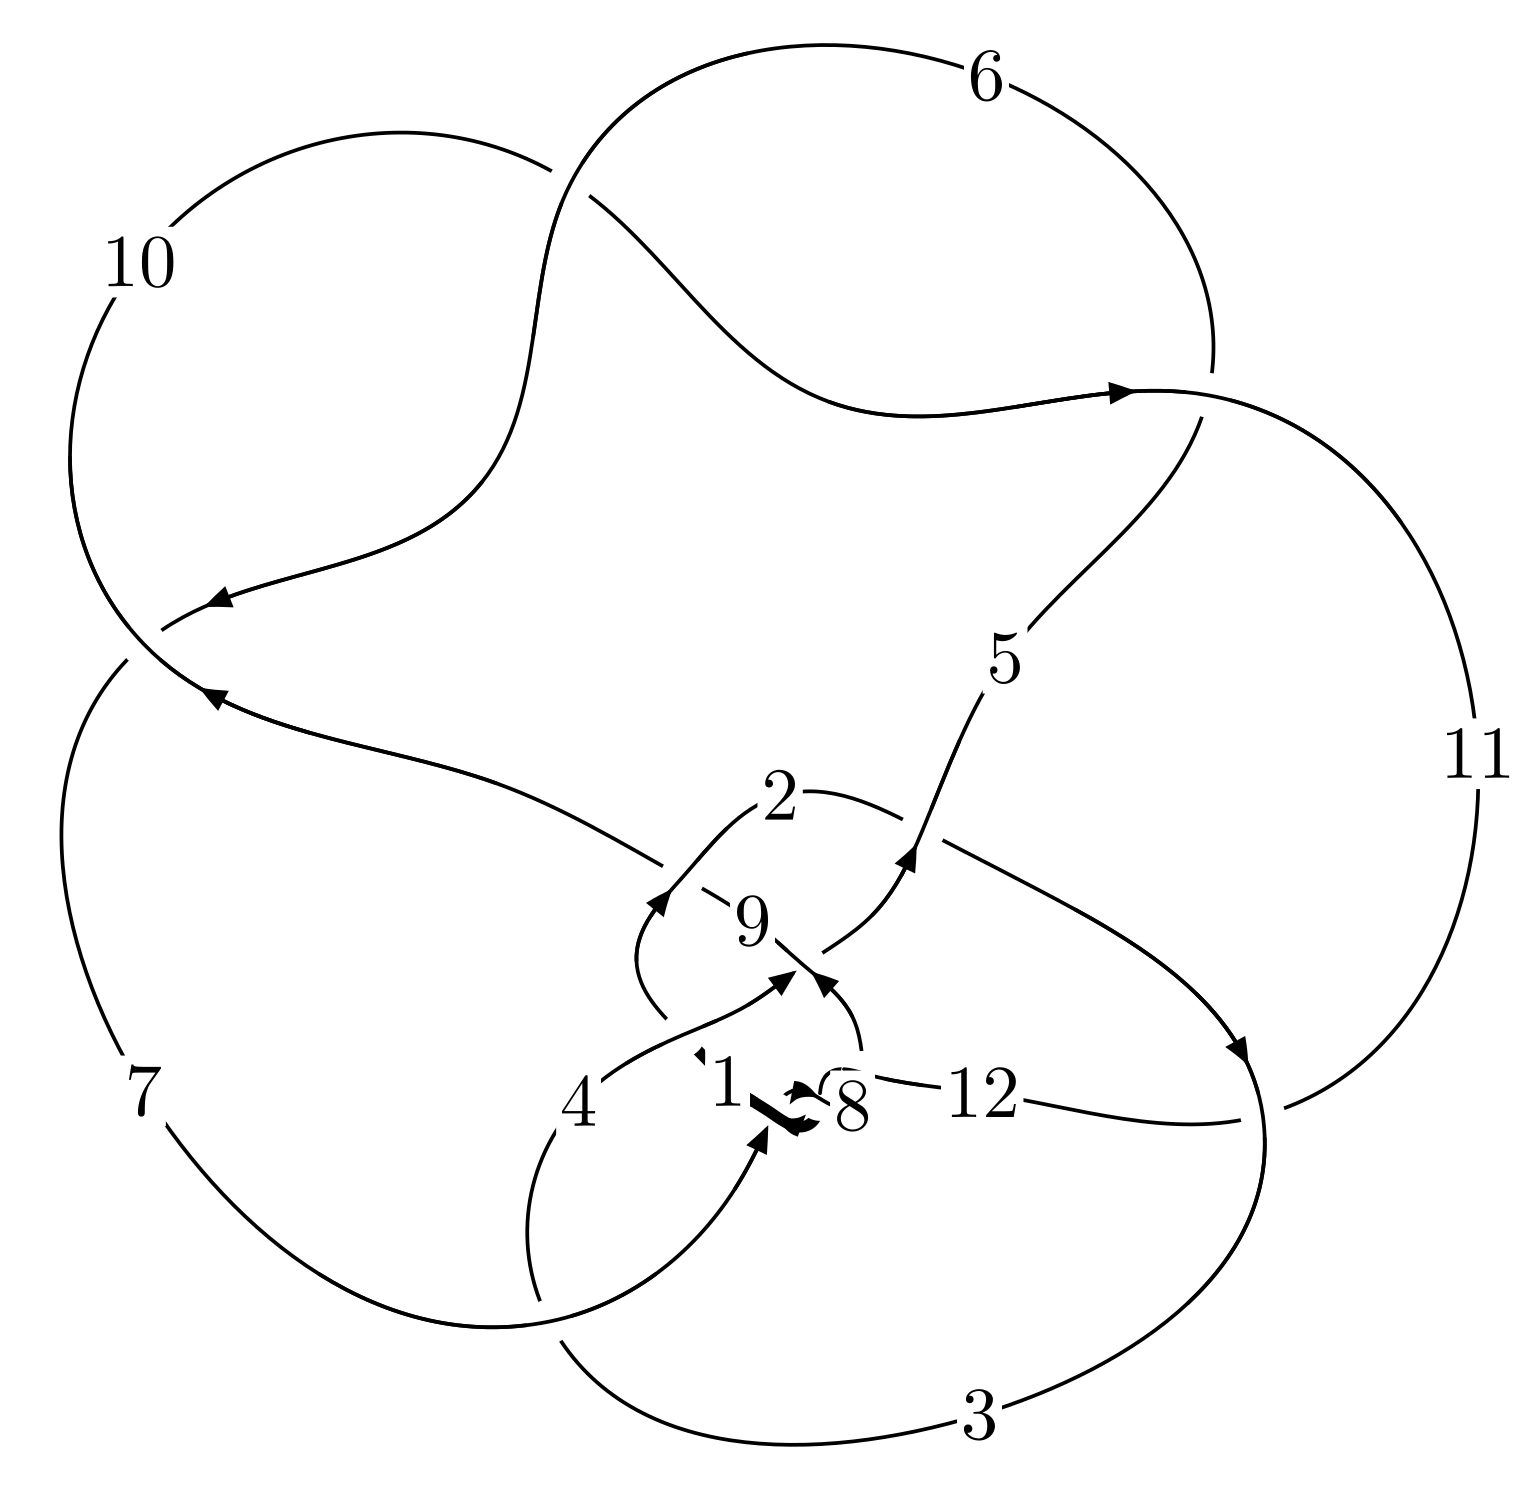
\includegraphics[width=112pt]{../../../GIT/diagram.site/Diagrams/png/1622_12a_0821.png}\\
\ \ \ A knot diagram\footnotemark}&
\allowdisplaybreaks
\textbf{Linearized knot diagam} \\
\cline{2-2}
 &
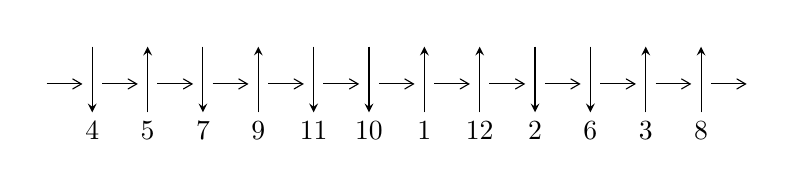
\begin{tikzpicture}[x=20pt, y=17pt]
	% nodes
	\node (C0) at (0, 0) {};
	\node (C1) at (1, 0) {};
	\node (C1U) at (1, +1) {};
	\node (C1D) at (1, -1) {4};

	\node (C2) at (2, 0) {};
	\node (C2U) at (2, +1) {};
	\node (C2D) at (2, -1) {5};

	\node (C3) at (3, 0) {};
	\node (C3U) at (3, +1) {};
	\node (C3D) at (3, -1) {7};

	\node (C4) at (4, 0) {};
	\node (C4U) at (4, +1) {};
	\node (C4D) at (4, -1) {9};

	\node (C5) at (5, 0) {};
	\node (C5U) at (5, +1) {};
	\node (C5D) at (5, -1) {11};

	\node (C6) at (6, 0) {};
	\node (C6U) at (6, +1) {};
	\node (C6D) at (6, -1) {10};

	\node (C7) at (7, 0) {};
	\node (C7U) at (7, +1) {};
	\node (C7D) at (7, -1) {1};

	\node (C8) at (8, 0) {};
	\node (C8U) at (8, +1) {};
	\node (C8D) at (8, -1) {12};

	\node (C9) at (9, 0) {};
	\node (C9U) at (9, +1) {};
	\node (C9D) at (9, -1) {2};

	\node (C10) at (10, 0) {};
	\node (C10U) at (10, +1) {};
	\node (C10D) at (10, -1) {6};

	\node (C11) at (11, 0) {};
	\node (C11U) at (11, +1) {};
	\node (C11D) at (11, -1) {3};

	\node (C12) at (12, 0) {};
	\node (C12U) at (12, +1) {};
	\node (C12D) at (12, -1) {8};
	\node (C13) at (13, 0) {};

	% arrows
	\draw[->,>={angle 60}]
	(C0) edge (C1) (C1) edge (C2) (C2) edge (C3) (C3) edge (C4) (C4) edge (C5) (C5) edge (C6) (C6) edge (C7) (C7) edge (C8) (C8) edge (C9) (C9) edge (C10) (C10) edge (C11) (C11) edge (C12) (C12) edge (C13) ;	\draw[->,>=stealth]
	(C1U) edge (C1D) (C2D) edge (C2U) (C3U) edge (C3D) (C4D) edge (C4U) (C5U) edge (C5D) (C6U) edge (C6D) (C7D) edge (C7U) (C8D) edge (C8U) (C9U) edge (C9D) (C10U) edge (C10D) (C11D) edge (C11U) (C12D) edge (C12U) ;
	\end{tikzpicture} \\
\hhline{~~} \\& 
\textbf{Solving Sequence} \\ \cline{2-2} 
 &
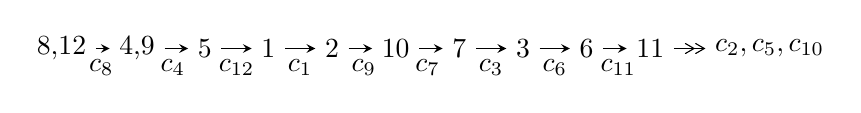
\begin{tikzpicture}[x=23pt, y=7pt]
	% node
	\node (A0) at (-1/8, 0) {8,12};
	\node (A1) at (17/16, 0) {4,9};
	\node (A2) at (17/8, 0) {5};
	\node (A3) at (25/8, 0) {1};
	\node (A4) at (33/8, 0) {2};
	\node (A5) at (41/8, 0) {10};
	\node (A6) at (49/8, 0) {7};
	\node (A7) at (57/8, 0) {3};
	\node (A8) at (65/8, 0) {6};
	\node (A9) at (73/8, 0) {11};
	\node (C1) at (1/2, -1) {$c_{8}$};
	\node (C2) at (13/8, -1) {$c_{4}$};
	\node (C3) at (21/8, -1) {$c_{12}$};
	\node (C4) at (29/8, -1) {$c_{1}$};
	\node (C5) at (37/8, -1) {$c_{9}$};
	\node (C6) at (45/8, -1) {$c_{7}$};
	\node (C7) at (53/8, -1) {$c_{3}$};
	\node (C8) at (61/8, -1) {$c_{6}$};
	\node (C9) at (69/8, -1) {$c_{11}$};
	\node (A10) at (11, 0) {$c_{2},c_{5},c_{10}$};

	% edge
	\draw[->,>=stealth]	
	(A0) edge (A1) (A1) edge (A2) (A2) edge (A3) (A3) edge (A4) (A4) edge (A5) (A5) edge (A6) (A6) edge (A7) (A7) edge (A8) (A8) edge (A9) ;
	\draw[->>,>={angle 60}]	
	(A9) edge (A10);
\end{tikzpicture} \\ 

\end{tabular} \\

\footnotetext{
The image of knot diagram is generated by the software ``\textbf{Draw programme}" developed by Andrew Bartholomew(\url{http://www.layer8.co.uk/maths/draw/index.htm\#Running-draw}), where we modified some parts for our purpose(\url{https://github.com/CATsTAILs/LinksPainter}).
}\phantom \\ \newline 
\centering \textbf{Ideals for irreducible components\footnotemark of $X_{\text{par}}$} 
 
\begin{align*}
I^u_{1}&=\langle 
1.72675\times10^{263} u^{121}+6.46926\times10^{262} u^{120}+\cdots+5.79158\times10^{262} b+2.48722\times10^{263},\\
\phantom{I^u_{1}}&\phantom{= \langle  }-8.49488\times10^{262} u^{121}-4.05282\times10^{262} u^{120}+\cdots+5.79158\times10^{262} a+1.38533\times10^{264},\\
\phantom{I^u_{1}}&\phantom{= \langle  }u^{122}+60 u^{120}+\cdots-18 u+1\rangle \\
I^u_{2}&=\langle 
1390 u^{25}-2769 u^{24}+\cdots+509 b-880,\;259 u^{25}-1267 u^{24}+\cdots+509 a-4214,\\
\phantom{I^u_{2}}&\phantom{= \langle  }u^{26}- u^{25}+\cdots-2 u+1\rangle \\
\\
\end{align*}
\raggedright * 2 irreducible components of $\dim_{\mathbb{C}}=0$, with total 148 representations.\\
\footnotetext{All coefficients of polynomials are rational numbers. But the coefficients are sometimes approximated in decimal forms when there is not enough margin.}
\newpage
\renewcommand{\arraystretch}{1}
\centering \section*{I. $I^u_{1}= \langle 1.73\times10^{263} u^{121}+6.47\times10^{262} u^{120}+\cdots+5.79\times10^{262} b+2.49\times10^{263},\;-8.49\times10^{262} u^{121}-4.05\times10^{262} u^{120}+\cdots+5.79\times10^{262} a+1.39\times10^{264},\;u^{122}+60 u^{120}+\cdots-18 u+1 \rangle$}
\flushleft \textbf{(i) Arc colorings}\\
\begin{tabular}{m{7pt} m{180pt} m{7pt} m{180pt} }
\flushright $a_{8}=$&$\begin{pmatrix}1\\0\end{pmatrix}$ \\
\flushright $a_{12}=$&$\begin{pmatrix}0\\u\end{pmatrix}$ \\
\flushright $a_{4}=$&$\begin{pmatrix}1.46676 u^{121}+0.699777 u^{120}+\cdots+170.001 u-23.9197\\-2.98148 u^{121}-1.11701 u^{120}+\cdots+45.9338 u-4.29454\end{pmatrix}$ \\
\flushright $a_{9}=$&$\begin{pmatrix}1\\- u^2\end{pmatrix}$ \\
\flushright $a_{5}=$&$\begin{pmatrix}1.77570 u^{121}-0.496966 u^{120}+\cdots+227.064 u-28.9140\\-4.01873 u^{121}-3.76337 u^{120}+\cdots+67.7841 u-5.49129\end{pmatrix}$ \\
\flushright $a_{1}=$&$\begin{pmatrix}u\\u\end{pmatrix}$ \\
\flushright $a_{2}=$&$\begin{pmatrix}8.98546 u^{121}+5.82372 u^{120}+\cdots+129.978 u-18.8375\\7.95443 u^{121}+7.03759 u^{120}+\cdots-157.645 u+8.82072\end{pmatrix}$ \\
\flushright $a_{10}=$&$\begin{pmatrix}-4.62391 u^{121}+3.55481 u^{120}+\cdots-46.0186 u+11.4590\\-7.69569 u^{121}+7.64762 u^{120}+\cdots-100.145 u+6.26253\end{pmatrix}$ \\
\flushright $a_{7}=$&$\begin{pmatrix}u^2+1\\u^2\end{pmatrix}$ \\
\flushright $a_{3}=$&$\begin{pmatrix}3.23207 u^{121}+0.625734 u^{120}+\cdots+214.441 u-27.8862\\-1.25329 u^{121}-2.67980 u^{120}+\cdots+72.6941 u-5.78329\end{pmatrix}$ \\
\flushright $a_{6}=$&$\begin{pmatrix}3.31846 u^{121}-6.79592 u^{120}+\cdots+310.776 u-24.6475\\-3.19180 u^{121}-13.6438 u^{120}+\cdots+200.032 u-12.4801\end{pmatrix}$ \\
\flushright $a_{11}=$&$\begin{pmatrix}-0.0220914 u^{121}-1.65462 u^{120}+\cdots+186.723 u-25.3586\\-2.95145 u^{121}-3.32993 u^{120}+\cdots+93.4416 u-6.90577\end{pmatrix}$\\&\end{tabular}
\flushleft \textbf{(ii) Obstruction class $= -1$}\\~\\
\flushleft \textbf{(iii) Cusp Shapes $= 4.67507 u^{121}+0.727293 u^{120}+\cdots+484.082 u-41.7114$}\\~\\
\newpage\renewcommand{\arraystretch}{1}
\flushleft \textbf{(iv) u-Polynomials at the component}\newline \\
\begin{tabular}{m{50pt}|m{274pt}}
Crossings & \hspace{64pt}u-Polynomials at each crossing \\
\hline $$\begin{aligned}c_{1}\end{aligned}$$&$\begin{aligned}
&u^{122}+4 u^{121}+\cdots-88956 u+26901
\end{aligned}$\\
\hline $$\begin{aligned}c_{2}\end{aligned}$$&$\begin{aligned}
&u^{122}-4 u^{121}+\cdots+88956 u+26901
\end{aligned}$\\
\hline $$\begin{aligned}c_{3}\end{aligned}$$&$\begin{aligned}
&u^{122}-2 u^{121}+\cdots+565031 u-52219
\end{aligned}$\\
\hline $$\begin{aligned}c_{4}\end{aligned}$$&$\begin{aligned}
&u^{122}+u^{121}+\cdots+68 u^2-1
\end{aligned}$\\
\hline $$\begin{aligned}c_{5},c_{6},c_{10}\end{aligned}$$&$\begin{aligned}
&u^{122}+60 u^{120}+\cdots+18 u+1
\end{aligned}$\\
\hline $$\begin{aligned}c_{7},c_{8},c_{12}\end{aligned}$$&$\begin{aligned}
&u^{122}+60 u^{120}+\cdots-18 u+1
\end{aligned}$\\
\hline $$\begin{aligned}c_{9}\end{aligned}$$&$\begin{aligned}
&u^{122}- u^{121}+\cdots+68 u^2-1
\end{aligned}$\\
\hline $$\begin{aligned}c_{11}\end{aligned}$$&$\begin{aligned}
&u^{122}+2 u^{121}+\cdots-565031 u-52219
\end{aligned}$\\
\hline
\end{tabular}\\~\\
\newpage\renewcommand{\arraystretch}{1}
\flushleft \textbf{(v) Riley Polynomials at the component}\newline \\
\begin{tabular}{m{50pt}|m{274pt}}
Crossings & \hspace{64pt}Riley Polynomials at each crossing \\
\hline $$\begin{aligned}c_{1},c_{2}\end{aligned}$$&$\begin{aligned}
&y^{122}-30 y^{121}+\cdots-23656173156 y+723663801
\end{aligned}$\\
\hline $$\begin{aligned}c_{3},c_{11}\end{aligned}$$&$\begin{aligned}
&y^{122}-18 y^{121}+\cdots-76906534499 y+2726823961
\end{aligned}$\\
\hline $$\begin{aligned}c_{4},c_{9}\end{aligned}$$&$\begin{aligned}
&y^{122}+21 y^{121}+\cdots-136 y+1
\end{aligned}$\\
\hline $$\begin{aligned}c_{5},c_{6},c_{7}\\c_{8},c_{10},c_{12}\end{aligned}$$&$\begin{aligned}
&y^{122}+120 y^{121}+\cdots-222 y+1
\end{aligned}$\\
\hline
\end{tabular}\\~\\
\newpage\flushleft \textbf{(vi) Complex Volumes and Cusp Shapes}
$$\begin{array}{c|c|c}  
\text{Solutions to }I^u_{1}& \I (\text{vol} + \sqrt{-1}CS) & \text{Cusp shape}\\
 \hline 
\begin{aligned}
u &= \phantom{-}0.838123 + 0.469947 I \\
a &= \phantom{-}0.818660 - 0.409892 I \\
b &= \phantom{-}0.283894 + 0.627860 I\end{aligned}
 & \phantom{-}0.76614 + 4.56382 I & \phantom{-0.000000 } 0 \\ \hline\begin{aligned}
u &= \phantom{-}0.838123 - 0.469947 I \\
a &= \phantom{-}0.818660 + 0.409892 I \\
b &= \phantom{-}0.283894 - 0.627860 I\end{aligned}
 & \phantom{-}0.76614 - 4.56382 I & \phantom{-0.000000 } 0 \\ \hline\begin{aligned}
u &= \phantom{-}0.841269 + 0.462133 I \\
a &= \phantom{-}0.777756 - 0.677243 I \\
b &= \phantom{-}0.178743 + 0.731523 I\end{aligned}
 & \phantom{-}6.3817 + 14.0924 I & \phantom{-0.000000 } 0 \\ \hline\begin{aligned}
u &= \phantom{-}0.841269 - 0.462133 I \\
a &= \phantom{-}0.777756 + 0.677243 I \\
b &= \phantom{-}0.178743 - 0.731523 I\end{aligned}
 & \phantom{-}6.3817 - 14.0924 I & \phantom{-0.000000 } 0 \\ \hline\begin{aligned}
u &= -0.838892 + 0.460556 I \\
a &= -0.832115 - 0.584852 I \\
b &= -0.209869 + 0.671328 I\end{aligned}
 & \phantom{-0.000000 } -9.93331 I & \phantom{-0.000000 } 0 \\ \hline\begin{aligned}
u &= -0.838892 - 0.460556 I \\
a &= -0.832115 + 0.584852 I \\
b &= -0.209869 - 0.671328 I\end{aligned}
 & \phantom{-0.000000 -}9.93331 I & \phantom{-0.000000 } 0 \\ \hline\begin{aligned}
u &= -0.748963 + 0.730792 I \\
a &= -0.403585 + 0.258143 I \\
b &= \phantom{-}0.458631 + 0.520460 I\end{aligned}
 & -0.76614 + 4.56382 I & \phantom{-0.000000 } 0 \\ \hline\begin{aligned}
u &= -0.748963 - 0.730792 I \\
a &= -0.403585 - 0.258143 I \\
b &= \phantom{-}0.458631 - 0.520460 I\end{aligned}
 & -0.76614 - 4.56382 I & \phantom{-0.000000 } 0 \\ \hline\begin{aligned}
u &= \phantom{-}0.765545 + 0.715335 I \\
a &= \phantom{-}0.417658 + 0.229663 I \\
b &= -0.593332 + 0.425549 I\end{aligned}
 & \phantom{-}5.65939 - 8.69735 I & \phantom{-0.000000 } 0 \\ \hline\begin{aligned}
u &= \phantom{-}0.765545 - 0.715335 I \\
a &= \phantom{-}0.417658 - 0.229663 I \\
b &= -0.593332 - 0.425549 I\end{aligned}
 & \phantom{-}5.65939 + 8.69735 I & \phantom{-0.000000 } 0\\
 \hline 
 \end{array}$$\newpage$$\begin{array}{c|c|c}  
\text{Solutions to }I^u_{1}& \I (\text{vol} + \sqrt{-1}CS) & \text{Cusp shape}\\
 \hline 
\begin{aligned}
u &= \phantom{-}0.753448 + 0.757254 I \\
a &= \phantom{-}0.452640 + 0.269754 I \\
b &= -0.155081 + 0.532232 I\end{aligned}
 & \phantom{-0.000000 -}0.859456 I & \phantom{-0.000000 } 0 \\ \hline\begin{aligned}
u &= \phantom{-}0.753448 - 0.757254 I \\
a &= \phantom{-}0.452640 - 0.269754 I \\
b &= -0.155081 - 0.532232 I\end{aligned}
 & \phantom{-0.000000 } -0.859456 I & \phantom{-0.000000 } 0 \\ \hline\begin{aligned}
u &= -0.791477 + 0.441571 I \\
a &= -0.533249 - 0.353695 I \\
b &= -0.410805 + 0.653910 I\end{aligned}
 & \phantom{-}8.75467 - 1.57080 I & \phantom{-0.000000 } 0 \\ \hline\begin{aligned}
u &= -0.791477 - 0.441571 I \\
a &= -0.533249 + 0.353695 I \\
b &= -0.410805 - 0.653910 I\end{aligned}
 & \phantom{-}8.75467 + 1.57080 I & \phantom{-0.000000 } 0 \\ \hline\begin{aligned}
u &= -0.503041 + 0.739634 I \\
a &= -0.336565 + 1.073680 I \\
b &= -0.015210 - 0.301055 I\end{aligned}
 & \phantom{-}3.72560 - 4.59585 I & \phantom{-0.000000 } 0 \\ \hline\begin{aligned}
u &= -0.503041 - 0.739634 I \\
a &= -0.336565 - 1.073680 I \\
b &= -0.015210 + 0.301055 I\end{aligned}
 & \phantom{-}3.72560 + 4.59585 I & \phantom{-0.000000 } 0 \\ \hline\begin{aligned}
u &= \phantom{-}0.774139 + 0.438683 I \\
a &= -0.226396 + 0.512883 I \\
b &= \phantom{-}0.159616 - 0.241386 I\end{aligned}
 & \phantom{-}0.68901 + 2.32956 I & \phantom{-0.000000 } 0 \\ \hline\begin{aligned}
u &= \phantom{-}0.774139 - 0.438683 I \\
a &= -0.226396 - 0.512883 I \\
b &= \phantom{-}0.159616 + 0.241386 I\end{aligned}
 & \phantom{-}0.68901 - 2.32956 I & \phantom{-0.000000 } 0 \\ \hline\begin{aligned}
u &= -0.823729 + 0.772937 I \\
a &= -0.297970 + 0.287398 I \\
b &= \phantom{-}0.0772759 - 0.0086507 I\end{aligned}
 & \phantom{-}7.93258 - 3.68575 I & \phantom{-0.000000 } 0 \\ \hline\begin{aligned}
u &= -0.823729 - 0.772937 I \\
a &= -0.297970 - 0.287398 I \\
b &= \phantom{-}0.0772759 + 0.0086507 I\end{aligned}
 & \phantom{-}7.93258 + 3.68575 I & \phantom{-0.000000 } 0\\
 \hline 
 \end{array}$$\newpage$$\begin{array}{c|c|c}  
\text{Solutions to }I^u_{1}& \I (\text{vol} + \sqrt{-1}CS) & \text{Cusp shape}\\
 \hline 
\begin{aligned}
u &= -0.197149 + 1.198090 I \\
a &= -0.391660 + 1.133070 I \\
b &= -0.066020 + 0.786727 I\end{aligned}
 & \phantom{-}2.05232 - 3.09473 I & \phantom{-0.000000 } 0 \\ \hline\begin{aligned}
u &= -0.197149 - 1.198090 I \\
a &= -0.391660 - 1.133070 I \\
b &= -0.066020 - 0.786727 I\end{aligned}
 & \phantom{-}2.05232 + 3.09473 I & \phantom{-0.000000 } 0 \\ \hline\begin{aligned}
u &= \phantom{-}0.368459 + 0.681988 I \\
a &= \phantom{-}0.333044 + 0.118458 I \\
b &= \phantom{-}0.411642 + 0.445181 I\end{aligned}
 & \phantom{-0.000000 -}1.64135 I & \phantom{-0.000000 } 0 \\ \hline\begin{aligned}
u &= \phantom{-}0.368459 - 0.681988 I \\
a &= \phantom{-}0.333044 - 0.118458 I \\
b &= \phantom{-}0.411642 - 0.445181 I\end{aligned}
 & \phantom{-0.000000 } -1.64135 I & \phantom{-0.000000 } 0 \\ \hline\begin{aligned}
u &= \phantom{-}0.088735 + 1.239840 I \\
a &= -1.085920 + 0.666668 I \\
b &= -0.097880 + 0.543491 I\end{aligned}
 & \phantom{-}4.34712 - 3.42917 I & \phantom{-0.000000 } 0 \\ \hline\begin{aligned}
u &= \phantom{-}0.088735 - 1.239840 I \\
a &= -1.085920 - 0.666668 I \\
b &= -0.097880 - 0.543491 I\end{aligned}
 & \phantom{-}4.34712 + 3.42917 I & \phantom{-0.000000 } 0 \\ \hline\begin{aligned}
u &= -0.746540 + 0.095924 I \\
a &= -0.179409 - 0.123127 I \\
b &= -0.869086 + 0.200995 I\end{aligned}
 & \phantom{-}5.88305 + 0.42236 I & \phantom{-0.000000 } 0 \\ \hline\begin{aligned}
u &= -0.746540 - 0.095924 I \\
a &= -0.179409 + 0.123127 I \\
b &= -0.869086 - 0.200995 I\end{aligned}
 & \phantom{-}5.88305 - 0.42236 I & \phantom{-0.000000 } 0 \\ \hline\begin{aligned}
u &= \phantom{-}0.003647 + 1.266340 I \\
a &= -0.29736 + 1.76121 I \\
b &= -0.56996 + 2.78197 I\end{aligned}
 & -1.52569 + 1.86247 I & \phantom{-0.000000 } 0 \\ \hline\begin{aligned}
u &= \phantom{-}0.003647 - 1.266340 I \\
a &= -0.29736 - 1.76121 I \\
b &= -0.56996 - 2.78197 I\end{aligned}
 & -1.52569 - 1.86247 I & \phantom{-0.000000 } 0\\
 \hline 
 \end{array}$$\newpage$$\begin{array}{c|c|c}  
\text{Solutions to }I^u_{1}& \I (\text{vol} + \sqrt{-1}CS) & \text{Cusp shape}\\
 \hline 
\begin{aligned}
u &= -1.002380 + 0.776849 I \\
a &= -0.120919 + 0.203444 I \\
b &= -0.0511940 - 0.0802179 I\end{aligned}
 & \phantom{-}7.91219 - 3.65289 I & \phantom{-0.000000 } 0 \\ \hline\begin{aligned}
u &= -1.002380 - 0.776849 I \\
a &= -0.120919 - 0.203444 I \\
b &= -0.0511940 + 0.0802179 I\end{aligned}
 & \phantom{-}7.91219 + 3.65289 I & \phantom{-0.000000 } 0 \\ \hline\begin{aligned}
u &= \phantom{-}0.011904 + 1.269570 I \\
a &= \phantom{-}0.64871 + 2.17404 I \\
b &= \phantom{-}1.19618 + 3.55643 I\end{aligned}
 & \phantom{-}4.40280 - 4.90152 I & \phantom{-0.000000 } 0 \\ \hline\begin{aligned}
u &= \phantom{-}0.011904 - 1.269570 I \\
a &= \phantom{-}0.64871 - 2.17404 I \\
b &= \phantom{-}1.19618 - 3.55643 I\end{aligned}
 & \phantom{-}4.40280 + 4.90152 I & \phantom{-0.000000 } 0 \\ \hline\begin{aligned}
u &= \phantom{-}0.126163 + 1.271520 I \\
a &= \phantom{-}0.026835 + 0.828486 I \\
b &= -0.674272 + 0.970458 I\end{aligned}
 & -2.39484 + 2.47343 I & \phantom{-0.000000 } 0 \\ \hline\begin{aligned}
u &= \phantom{-}0.126163 - 1.271520 I \\
a &= \phantom{-}0.026835 - 0.828486 I \\
b &= -0.674272 - 0.970458 I\end{aligned}
 & -2.39484 - 2.47343 I & \phantom{-0.000000 } 0 \\ \hline\begin{aligned}
u &= \phantom{-}0.387895 + 0.597696 I \\
a &= \phantom{-}0.165680 + 1.337830 I \\
b &= -0.149993 - 0.321583 I\end{aligned}
 & -1.18377 + 3.27789 I & -7.72431 - 9.92436 I \\ \hline\begin{aligned}
u &= \phantom{-}0.387895 - 0.597696 I \\
a &= \phantom{-}0.165680 - 1.337830 I \\
b &= -0.149993 + 0.321583 I\end{aligned}
 & -1.18377 - 3.27789 I & -7.72431 + 9.92436 I \\ \hline\begin{aligned}
u &= \phantom{-}0.034387 + 1.288040 I \\
a &= \phantom{-}0.469851 + 0.313970 I \\
b &= -0.454940 + 0.131391 I\end{aligned}
 & -2.11977 + 2.41437 I & \phantom{-0.000000 } 0 \\ \hline\begin{aligned}
u &= \phantom{-}0.034387 - 1.288040 I \\
a &= \phantom{-}0.469851 - 0.313970 I \\
b &= -0.454940 - 0.131391 I\end{aligned}
 & -2.11977 - 2.41437 I & \phantom{-0.000000 } 0\\
 \hline 
 \end{array}$$\newpage$$\begin{array}{c|c|c}  
\text{Solutions to }I^u_{1}& \I (\text{vol} + \sqrt{-1}CS) & \text{Cusp shape}\\
 \hline 
\begin{aligned}
u &= \phantom{-}0.591507 + 0.393541 I \\
a &= -0.692120 + 0.928039 I \\
b &= \phantom{-}0.454824 - 0.527439 I\end{aligned}
 & \phantom{-}1.52569 + 1.86247 I & \phantom{-0.000000 } 0 \\ \hline\begin{aligned}
u &= \phantom{-}0.591507 - 0.393541 I \\
a &= -0.692120 - 0.928039 I \\
b &= \phantom{-}0.454824 + 0.527439 I\end{aligned}
 & \phantom{-}1.52569 - 1.86247 I & \phantom{-0.000000 } 0 \\ \hline\begin{aligned}
u &= -0.559765 + 0.386642 I \\
a &= \phantom{-}0.475141 + 1.153770 I \\
b &= -0.108108 - 0.733708 I\end{aligned}
 & -1.67571 - 3.29126 I & -7.51122 + 8.90970 I \\ \hline\begin{aligned}
u &= -0.559765 - 0.386642 I \\
a &= \phantom{-}0.475141 - 1.153770 I \\
b &= -0.108108 + 0.733708 I\end{aligned}
 & -1.67571 + 3.29126 I & -7.51122 - 8.90970 I \\ \hline\begin{aligned}
u &= \phantom{-}0.668209\phantom{ +0.000000I} \\
a &= \phantom{-}0.293080\phantom{ +0.000000I} \\
b &= \phantom{-}0.741541\phantom{ +0.000000I}\end{aligned}
 & \phantom{-}1.02756\phantom{ +0.000000I} & \phantom{-}9.74990\phantom{ +0.000000I} \\ \hline\begin{aligned}
u &= -0.223878 + 1.319960 I \\
a &= \phantom{-}0.348405 + 1.026390 I \\
b &= \phantom{-}1.14248 + 1.74084 I\end{aligned}
 & \phantom{-}1.94229 + 0.21639 I & \phantom{-0.000000 } 0 \\ \hline\begin{aligned}
u &= -0.223878 - 1.319960 I \\
a &= \phantom{-}0.348405 - 1.026390 I \\
b &= \phantom{-}1.14248 - 1.74084 I\end{aligned}
 & \phantom{-}1.94229 - 0.21639 I & \phantom{-0.000000 } 0 \\ \hline\begin{aligned}
u &= \phantom{-}0.094887 + 1.340650 I \\
a &= -0.54452 - 2.88908 I \\
b &= -0.85968 - 3.19953 I\end{aligned}
 & \phantom{-}3.76570 + 7.21033 I & \phantom{-0.000000 } 0 \\ \hline\begin{aligned}
u &= \phantom{-}0.094887 - 1.340650 I \\
a &= -0.54452 + 2.88908 I \\
b &= -0.85968 + 3.19953 I\end{aligned}
 & \phantom{-}3.76570 - 7.21033 I & \phantom{-0.000000 } 0 \\ \hline\begin{aligned}
u &= \phantom{-}0.572996 + 0.313961 I \\
a &= -0.573007 + 1.232680 I \\
b &= \phantom{-}0.029546 - 1.023280 I\end{aligned}
 & \phantom{-}2.97533 + 5.05203 I & \phantom{-}2.55990 - 8.99574 I\\
 \hline 
 \end{array}$$\newpage$$\begin{array}{c|c|c}  
\text{Solutions to }I^u_{1}& \I (\text{vol} + \sqrt{-1}CS) & \text{Cusp shape}\\
 \hline 
\begin{aligned}
u &= \phantom{-}0.572996 - 0.313961 I \\
a &= -0.573007 - 1.232680 I \\
b &= \phantom{-}0.029546 + 1.023280 I\end{aligned}
 & \phantom{-}2.97533 - 5.05203 I & \phantom{-}2.55990 + 8.99574 I \\ \hline\begin{aligned}
u &= \phantom{-}0.211626 + 0.612080 I \\
a &= -0.181398 + 0.533514 I \\
b &= -0.45860 + 1.36493 I\end{aligned}
 & -0.68901 + 2.32956 I & -6.85361 - 8.80115 I \\ \hline\begin{aligned}
u &= \phantom{-}0.211626 - 0.612080 I \\
a &= -0.181398 - 0.533514 I \\
b &= -0.45860 - 1.36493 I\end{aligned}
 & -0.68901 - 2.32956 I & -6.85361 + 8.80115 I \\ \hline\begin{aligned}
u &= \phantom{-}0.281078 + 1.336330 I \\
a &= \phantom{-}0.930616 - 0.634656 I \\
b &= \phantom{-}1.29676 - 1.30744 I\end{aligned}
 & -1.94229 + 0.21639 I & \phantom{-0.000000 } 0 \\ \hline\begin{aligned}
u &= \phantom{-}0.281078 - 1.336330 I \\
a &= \phantom{-}0.930616 + 0.634656 I \\
b &= \phantom{-}1.29676 + 1.30744 I\end{aligned}
 & -1.94229 - 0.21639 I & \phantom{-0.000000 } 0 \\ \hline\begin{aligned}
u &= -0.102970 + 1.365190 I \\
a &= \phantom{-}0.555873 + 0.182955 I \\
b &= \phantom{-}2.00596 + 0.29788 I\end{aligned}
 & -2.97533 - 5.05203 I & \phantom{-0.000000 } 0 \\ \hline\begin{aligned}
u &= -0.102970 - 1.365190 I \\
a &= \phantom{-}0.555873 - 0.182955 I \\
b &= \phantom{-}2.00596 - 0.29788 I\end{aligned}
 & -2.97533 + 5.05203 I & \phantom{-0.000000 } 0 \\ \hline\begin{aligned}
u &= -0.597169 + 0.203460 I \\
a &= -2.29060 - 0.07482 I \\
b &= -0.219353 - 0.076676 I\end{aligned}
 & \phantom{-}6.69507 + 3.24081 I & \phantom{-}7.82762 - 0.48317 I \\ \hline\begin{aligned}
u &= -0.597169 - 0.203460 I \\
a &= -2.29060 + 0.07482 I \\
b &= -0.219353 + 0.076676 I\end{aligned}
 & \phantom{-}6.69507 - 3.24081 I & \phantom{-}7.82762 + 0.48317 I \\ \hline\begin{aligned}
u &= -0.405018 + 0.468237 I \\
a &= \phantom{-}0.292180 + 0.281700 I \\
b &= \phantom{-}0.72718 + 1.42275 I\end{aligned}
 & \phantom{-}5.62384 - 6.30894 I & \phantom{-}0.86595 + 10.40267 I\\
 \hline 
 \end{array}$$\newpage$$\begin{array}{c|c|c}  
\text{Solutions to }I^u_{1}& \I (\text{vol} + \sqrt{-1}CS) & \text{Cusp shape}\\
 \hline 
\begin{aligned}
u &= -0.405018 - 0.468237 I \\
a &= \phantom{-}0.292180 - 0.281700 I \\
b &= \phantom{-}0.72718 - 1.42275 I\end{aligned}
 & \phantom{-}5.62384 + 6.30894 I & \phantom{-}0.86595 - 10.40267 I \\ \hline\begin{aligned}
u &= \phantom{-}0.016831 + 1.382940 I \\
a &= \phantom{-}0.366374 - 0.827698 I \\
b &= -0.61848 - 1.46951 I\end{aligned}
 & -2.05232 + 3.09473 I & \phantom{-0.000000 } 0 \\ \hline\begin{aligned}
u &= \phantom{-}0.016831 - 1.382940 I \\
a &= \phantom{-}0.366374 + 0.827698 I \\
b &= -0.61848 + 1.46951 I\end{aligned}
 & -2.05232 - 3.09473 I & \phantom{-0.000000 } 0 \\ \hline\begin{aligned}
u &= \phantom{-}0.118092 + 1.386860 I \\
a &= -0.907334 + 0.319639 I \\
b &= -2.59599 + 0.67827 I\end{aligned}
 & \phantom{-}2.63743 + 7.92429 I & \phantom{-0.000000 } 0 \\ \hline\begin{aligned}
u &= \phantom{-}0.118092 - 1.386860 I \\
a &= -0.907334 - 0.319639 I \\
b &= -2.59599 - 0.67827 I\end{aligned}
 & \phantom{-}2.63743 - 7.92429 I & \phantom{-0.000000 } 0 \\ \hline\begin{aligned}
u &= -0.078291 + 1.391230 I \\
a &= \phantom{-}0.92867 - 2.35012 I \\
b &= \phantom{-}1.01328 - 2.92847 I\end{aligned}
 & -3.72560 - 4.59585 I & \phantom{-0.000000 } 0 \\ \hline\begin{aligned}
u &= -0.078291 - 1.391230 I \\
a &= \phantom{-}0.92867 + 2.35012 I \\
b &= \phantom{-}1.01328 + 2.92847 I\end{aligned}
 & -3.72560 + 4.59585 I & \phantom{-0.000000 } 0 \\ \hline\begin{aligned}
u &= \phantom{-}0.033130 + 1.400890 I \\
a &= -1.05242 - 1.46627 I \\
b &= -0.63083 - 2.14230 I\end{aligned}
 & -5.88305 + 0.42236 I & \phantom{-0.000000 } 0 \\ \hline\begin{aligned}
u &= \phantom{-}0.033130 - 1.400890 I \\
a &= -1.05242 + 1.46627 I \\
b &= -0.63083 + 2.14230 I\end{aligned}
 & -5.88305 - 0.42236 I & \phantom{-0.000000 } 0 \\ \hline\begin{aligned}
u &= \phantom{-}0.21145 + 1.42791 I \\
a &= \phantom{-}0.15300 - 2.14751 I \\
b &= -0.57741 - 3.21135 I\end{aligned}
 & -2.63743 + 7.92429 I & \phantom{-0.000000 } 0\\
 \hline 
 \end{array}$$\newpage$$\begin{array}{c|c|c}  
\text{Solutions to }I^u_{1}& \I (\text{vol} + \sqrt{-1}CS) & \text{Cusp shape}\\
 \hline 
\begin{aligned}
u &= \phantom{-}0.21145 - 1.42791 I \\
a &= \phantom{-}0.15300 + 2.14751 I \\
b &= -0.57741 + 3.21135 I\end{aligned}
 & -2.63743 - 7.92429 I & \phantom{-0.000000 } 0 \\ \hline\begin{aligned}
u &= -0.28430 + 1.41809 I \\
a &= -0.611540 - 1.008500 I \\
b &= -0.62489 - 1.88264 I\end{aligned}
 & -6.69507 - 3.24081 I & \phantom{-0.000000 } 0 \\ \hline\begin{aligned}
u &= -0.28430 - 1.41809 I \\
a &= -0.611540 + 1.008500 I \\
b &= -0.62489 + 1.88264 I\end{aligned}
 & -6.69507 + 3.24081 I & \phantom{-0.000000 } 0 \\ \hline\begin{aligned}
u &= -0.512822 + 0.202337 I \\
a &= \phantom{-}1.029400 + 0.201671 I \\
b &= -0.507931 - 0.117189 I\end{aligned}
 & -1.54857 + 0.09873 I & -6.52365 + 0.22723 I \\ \hline\begin{aligned}
u &= -0.512822 - 0.202337 I \\
a &= \phantom{-}1.029400 - 0.201671 I \\
b &= -0.507931 + 0.117189 I\end{aligned}
 & -1.54857 - 0.09873 I & -6.52365 - 0.22723 I \\ \hline\begin{aligned}
u &= \phantom{-}0.541620 + 0.049842 I \\
a &= \phantom{-}1.57917 + 0.46289 I \\
b &= \phantom{-}0.395132 - 0.075128 I\end{aligned}
 & \phantom{-}1.54857 + 0.09873 I & \phantom{-}6.52365 + 0.22723 I \\ \hline\begin{aligned}
u &= \phantom{-}0.541620 - 0.049842 I \\
a &= \phantom{-}1.57917 - 0.46289 I \\
b &= \phantom{-}0.395132 + 0.075128 I\end{aligned}
 & \phantom{-}1.54857 - 0.09873 I & \phantom{-}6.52365 - 0.22723 I \\ \hline\begin{aligned}
u &= -0.20934 + 1.45200 I \\
a &= -0.15208 - 1.90295 I \\
b &= \phantom{-}0.41340 - 3.02350 I\end{aligned}
 & -7.61338 - 6.13503 I & \phantom{-0.000000 } 0 \\ \hline\begin{aligned}
u &= -0.20934 - 1.45200 I \\
a &= -0.15208 + 1.90295 I \\
b &= \phantom{-}0.41340 + 3.02350 I\end{aligned}
 & -7.61338 + 6.13503 I & \phantom{-0.000000 } 0 \\ \hline\begin{aligned}
u &= \phantom{-}0.22745 + 1.45151 I \\
a &= \phantom{-}0.50169 - 1.70373 I \\
b &= \phantom{-}0.15167 - 2.99070 I\end{aligned}
 & -4.40280 + 4.90152 I & \phantom{-0.000000 } 0\\
 \hline 
 \end{array}$$\newpage$$\begin{array}{c|c|c}  
\text{Solutions to }I^u_{1}& \I (\text{vol} + \sqrt{-1}CS) & \text{Cusp shape}\\
 \hline 
\begin{aligned}
u &= \phantom{-}0.22745 - 1.45151 I \\
a &= \phantom{-}0.50169 + 1.70373 I \\
b &= \phantom{-}0.15167 + 2.99070 I\end{aligned}
 & -4.40280 - 4.90152 I & \phantom{-0.000000 } 0 \\ \hline\begin{aligned}
u &= -0.14721 + 1.47595 I \\
a &= \phantom{-}1.43924 + 1.51730 I \\
b &= \phantom{-}1.07349 + 1.98141 I\end{aligned}
 & -0.68291 - 8.38710 I & \phantom{-0.000000 } 0 \\ \hline\begin{aligned}
u &= -0.14721 - 1.47595 I \\
a &= \phantom{-}1.43924 - 1.51730 I \\
b &= \phantom{-}1.07349 - 1.98141 I\end{aligned}
 & -0.68291 + 8.38710 I & \phantom{-0.000000 } 0 \\ \hline\begin{aligned}
u &= -0.10313 + 1.48416 I \\
a &= \phantom{-}0.51809 - 1.85788 I \\
b &= \phantom{-}0.81572 - 3.00333 I\end{aligned}
 & -4.34712 - 3.42917 I & \phantom{-0.000000 } 0 \\ \hline\begin{aligned}
u &= -0.10313 - 1.48416 I \\
a &= \phantom{-}0.51809 + 1.85788 I \\
b &= \phantom{-}0.81572 + 3.00333 I\end{aligned}
 & -4.34712 + 3.42917 I & \phantom{-0.000000 } 0 \\ \hline\begin{aligned}
u &= \phantom{-}0.15950 + 1.50706 I \\
a &= -0.33921 - 1.69479 I \\
b &= -0.84449 - 2.79461 I\end{aligned}
 & -8.01760 + 5.44098 I & \phantom{-0.000000 } 0 \\ \hline\begin{aligned}
u &= \phantom{-}0.15950 - 1.50706 I \\
a &= -0.33921 + 1.69479 I \\
b &= -0.84449 + 2.79461 I\end{aligned}
 & -8.01760 - 5.44098 I & \phantom{-0.000000 } 0 \\ \hline\begin{aligned}
u &= -0.003564 + 0.481131 I \\
a &= -0.90114 + 2.00705 I \\
b &= \phantom{-}0.593963 - 0.134342 I\end{aligned}
 & \phantom{-}2.11977 - 2.41437 I & -0.417958 + 1.258564 I \\ \hline\begin{aligned}
u &= -0.003564 - 0.481131 I \\
a &= -0.90114 - 2.00705 I \\
b &= \phantom{-}0.593963 + 0.134342 I\end{aligned}
 & \phantom{-}2.11977 + 2.41437 I & -0.417958 - 1.258564 I \\ \hline\begin{aligned}
u &= -0.27675 + 1.49874 I \\
a &= -0.03087 + 1.71174 I \\
b &= -0.37690 + 2.36519 I\end{aligned}
 & \phantom{-}2.46634 - 5.42668 I & \phantom{-0.000000 } 0\\
 \hline 
 \end{array}$$\newpage$$\begin{array}{c|c|c}  
\text{Solutions to }I^u_{1}& \I (\text{vol} + \sqrt{-1}CS) & \text{Cusp shape}\\
 \hline 
\begin{aligned}
u &= -0.27675 - 1.49874 I \\
a &= -0.03087 - 1.71174 I \\
b &= -0.37690 - 2.36519 I\end{aligned}
 & \phantom{-}2.46634 + 5.42668 I & \phantom{-0.000000 } 0 \\ \hline\begin{aligned}
u &= \phantom{-}0.29702 + 1.50535 I \\
a &= \phantom{-}0.093957 - 1.028920 I \\
b &= -0.26440 - 1.78844 I\end{aligned}
 & -5.62384 + 6.30894 I & \phantom{-0.000000 } 0 \\ \hline\begin{aligned}
u &= \phantom{-}0.29702 - 1.50535 I \\
a &= \phantom{-}0.093957 + 1.028920 I \\
b &= -0.26440 + 1.78844 I\end{aligned}
 & -5.62384 - 6.30894 I & \phantom{-0.000000 } 0 \\ \hline\begin{aligned}
u &= -0.30513 + 1.51162 I \\
a &= \phantom{-}0.01748 + 1.82265 I \\
b &= -0.37240 + 2.83356 I\end{aligned}
 & -6.3817 - 14.0924 I & \phantom{-0.000000 } 0 \\ \hline\begin{aligned}
u &= -0.30513 - 1.51162 I \\
a &= \phantom{-}0.01748 - 1.82265 I \\
b &= -0.37240 - 2.83356 I\end{aligned}
 & -6.3817 + 14.0924 I & \phantom{-0.000000 } 0 \\ \hline\begin{aligned}
u &= \phantom{-}0.30803 + 1.51176 I \\
a &= -0.00101 + 1.85616 I \\
b &= \phantom{-}0.48528 + 2.90856 I\end{aligned}
 & \phantom{-0.000000 -}18.2741 I & \phantom{-0.000000 } 0 \\ \hline\begin{aligned}
u &= \phantom{-}0.30803 - 1.51176 I \\
a &= -0.00101 - 1.85616 I \\
b &= \phantom{-}0.48528 - 2.90856 I\end{aligned}
 & \phantom{-0.000000 } -18.2741 I & \phantom{-0.000000 } 0 \\ \hline\begin{aligned}
u &= \phantom{-}0.30070 + 1.51406 I \\
a &= -0.01505 + 1.77596 I \\
b &= \phantom{-}0.28514 + 2.67352 I\end{aligned}
 & -5.65939 + 8.69735 I & \phantom{-0.000000 } 0 \\ \hline\begin{aligned}
u &= \phantom{-}0.30070 - 1.51406 I \\
a &= -0.01505 - 1.77596 I \\
b &= \phantom{-}0.28514 - 2.67352 I\end{aligned}
 & -5.65939 - 8.69735 I & \phantom{-0.000000 } 0 \\ \hline\begin{aligned}
u &= \phantom{-}0.444045 + 0.017440 I \\
a &= -1.054550 + 0.880836 I \\
b &= -0.80489 - 1.30581 I\end{aligned}
 & \phantom{-}8.01760 + 5.44098 I & \phantom{-}11.84308 - 5.29398 I\\
 \hline 
 \end{array}$$\newpage$$\begin{array}{c|c|c}  
\text{Solutions to }I^u_{1}& \I (\text{vol} + \sqrt{-1}CS) & \text{Cusp shape}\\
 \hline 
\begin{aligned}
u &= \phantom{-}0.444045 - 0.017440 I \\
a &= -1.054550 - 0.880836 I \\
b &= -0.80489 + 1.30581 I\end{aligned}
 & \phantom{-}8.01760 - 5.44098 I & \phantom{-}11.84308 + 5.29398 I \\ \hline\begin{aligned}
u &= \phantom{-}0.14067 + 1.55284 I \\
a &= -0.54774 + 1.69963 I \\
b &= -0.41708 + 2.22737 I\end{aligned}
 & -7.93258 + 3.68575 I & \phantom{-0.000000 } 0 \\ \hline\begin{aligned}
u &= \phantom{-}0.14067 - 1.55284 I \\
a &= -0.54774 - 1.69963 I \\
b &= -0.41708 - 2.22737 I\end{aligned}
 & -7.93258 - 3.68575 I & \phantom{-0.000000 } 0 \\ \hline\begin{aligned}
u &= -0.18374 + 1.55311 I \\
a &= \phantom{-}0.40161 - 1.45606 I \\
b &= \phantom{-}1.04761 - 2.52368 I\end{aligned}
 & -3.76570 - 7.21033 I & \phantom{-0.000000 } 0 \\ \hline\begin{aligned}
u &= -0.18374 - 1.55311 I \\
a &= \phantom{-}0.40161 + 1.45606 I \\
b &= \phantom{-}1.04761 + 2.52368 I\end{aligned}
 & -3.76570 + 7.21033 I & \phantom{-0.000000 } 0 \\ \hline\begin{aligned}
u &= \phantom{-}0.10216 + 1.56588 I \\
a &= -0.55103 + 2.11116 I \\
b &= -0.44359 + 2.57907 I\end{aligned}
 & -7.91219 + 3.65289 I & \phantom{-0.000000 } 0 \\ \hline\begin{aligned}
u &= \phantom{-}0.10216 - 1.56588 I \\
a &= -0.55103 - 2.11116 I \\
b &= -0.44359 - 2.57907 I\end{aligned}
 & -7.91219 - 3.65289 I & \phantom{-0.000000 } 0 \\ \hline\begin{aligned}
u &= -0.414540 + 0.099845 I \\
a &= -2.31360 + 2.12787 I \\
b &= -0.436622 - 0.246341 I\end{aligned}
 & \phantom{-}1.67571 - 3.29126 I & \phantom{-}7.51122 + 8.90970 I \\ \hline\begin{aligned}
u &= -0.414540 - 0.099845 I \\
a &= -2.31360 - 2.12787 I \\
b &= -0.436622 + 0.246341 I\end{aligned}
 & \phantom{-}1.67571 + 3.29126 I & \phantom{-}7.51122 - 8.90970 I \\ \hline\begin{aligned}
u &= -0.13898 + 1.57065 I \\
a &= \phantom{-}0.520682 + 1.204410 I \\
b &= \phantom{-}0.44191 + 1.80330 I\end{aligned}
 & -8.75467 + 1.57080 I & \phantom{-0.000000 } 0\\
 \hline 
 \end{array}$$\newpage$$\begin{array}{c|c|c}  
\text{Solutions to }I^u_{1}& \I (\text{vol} + \sqrt{-1}CS) & \text{Cusp shape}\\
 \hline 
\begin{aligned}
u &= -0.13898 - 1.57065 I \\
a &= \phantom{-}0.520682 - 1.204410 I \\
b &= \phantom{-}0.44191 - 1.80330 I\end{aligned}
 & -8.75467 - 1.57080 I & \phantom{-0.000000 } 0 \\ \hline\begin{aligned}
u &= \phantom{-}0.381622 + 0.153038 I \\
a &= \phantom{-}3.74983 + 2.22249 I \\
b &= \phantom{-}0.396790 - 0.342833 I\end{aligned}
 & \phantom{-}7.61338 + 6.13503 I & \phantom{-}12.1450 - 9.8024 I \\ \hline\begin{aligned}
u &= \phantom{-}0.381622 - 0.153038 I \\
a &= \phantom{-}3.74983 - 2.22249 I \\
b &= \phantom{-}0.396790 + 0.342833 I\end{aligned}
 & \phantom{-}7.61338 - 6.13503 I & \phantom{-}12.1450 + 9.8024 I \\ \hline\begin{aligned}
u &= -0.33714 + 1.56324 I \\
a &= \phantom{-}0.107214 - 0.797190 I \\
b &= \phantom{-}0.57846 - 1.34433 I\end{aligned}
 & \phantom{-}0.68291 - 8.38710 I & \phantom{-0.000000 } 0 \\ \hline\begin{aligned}
u &= -0.33714 - 1.56324 I \\
a &= \phantom{-}0.107214 + 0.797190 I \\
b &= \phantom{-}0.57846 + 1.34433 I\end{aligned}
 & \phantom{-}0.68291 + 8.38710 I & \phantom{-0.000000 } 0 \\ \hline\begin{aligned}
u &= \phantom{-}0.13250 + 1.60991 I \\
a &= -0.471533 + 0.981639 I \\
b &= -0.45579 + 1.59734 I\end{aligned}
 & -2.46634 - 5.42668 I & \phantom{-0.000000 } 0 \\ \hline\begin{aligned}
u &= \phantom{-}0.13250 - 1.60991 I \\
a &= -0.471533 - 0.981639 I \\
b &= -0.45579 - 1.59734 I\end{aligned}
 & -2.46634 + 5.42668 I & \phantom{-0.000000 } 0 \\ \hline\begin{aligned}
u &= -0.313695 + 0.118779 I \\
a &= \phantom{-}1.43384 + 1.57346 I \\
b &= \phantom{-}0.864812 - 0.896168 I\end{aligned}
 & \phantom{-}1.18377 - 3.27789 I & \phantom{-}7.72431 + 9.92436 I \\ \hline\begin{aligned}
u &= -0.313695 - 0.118779 I \\
a &= \phantom{-}1.43384 - 1.57346 I \\
b &= \phantom{-}0.864812 + 0.896168 I\end{aligned}
 & \phantom{-}1.18377 + 3.27789 I & \phantom{-}7.72431 - 9.92436 I \\ \hline\begin{aligned}
u &= \phantom{-}0.317523 + 0.085220 I \\
a &= -2.52056 - 1.69319 I \\
b &= \phantom{-}0.666836 + 0.066192 I\end{aligned}
 & \phantom{-}2.39484 - 2.47343 I & \phantom{-}1.59037 + 1.05433 I\\
 \hline 
 \end{array}$$\newpage$$\begin{array}{c|c|c}  
\text{Solutions to }I^u_{1}& \I (\text{vol} + \sqrt{-1}CS) & \text{Cusp shape}\\
 \hline 
\begin{aligned}
u &= \phantom{-}0.317523 - 0.085220 I \\
a &= -2.52056 + 1.69319 I \\
b &= \phantom{-}0.666836 - 0.066192 I\end{aligned}
 & \phantom{-}2.39484 + 2.47343 I & \phantom{-}1.59037 - 1.05433 I \\ \hline\begin{aligned}
u &= \phantom{-}0.0747499\phantom{ +0.000000I} \\
a &= -11.4868\phantom{ +0.000000I} \\
b &= -1.16381\phantom{ +0.000000I}\end{aligned}
 & -1.02756\phantom{ +0.000000I} & -9.74990\phantom{ +0.000000I}\\
 \hline 
 \end{array}$$\newpage\newpage\renewcommand{\arraystretch}{1}
\centering \section*{II. $I^u_{2}= \langle 1390 u^{25}-2769 u^{24}+\cdots+509 b-880,\;259 u^{25}-1267 u^{24}+\cdots+509 a-4214,\;u^{26}- u^{25}+\cdots-2 u+1 \rangle$}
\flushleft \textbf{(i) Arc colorings}\\
\begin{tabular}{m{7pt} m{180pt} m{7pt} m{180pt} }
\flushright $a_{8}=$&$\begin{pmatrix}1\\0\end{pmatrix}$ \\
\flushright $a_{12}=$&$\begin{pmatrix}0\\u\end{pmatrix}$ \\
\flushright $a_{4}=$&$\begin{pmatrix}-0.508841 u^{25}+2.48919 u^{24}+\cdots-13.5324 u+8.27898\\-2.73084 u^{25}+5.44008 u^{24}+\cdots-10.6798 u+1.72888\end{pmatrix}$ \\
\flushright $a_{9}=$&$\begin{pmatrix}1\\- u^2\end{pmatrix}$ \\
\flushright $a_{5}=$&$\begin{pmatrix}-2.83890 u^{25}+5.75246 u^{24}+\cdots-19.7426 u+8.02750\\-5.69352 u^{25}+10.0413 u^{24}+\cdots-14.8762 u+2.66208\end{pmatrix}$ \\
\flushright $a_{1}=$&$\begin{pmatrix}u\\u\end{pmatrix}$ \\
\flushright $a_{2}=$&$\begin{pmatrix}1.79961 u^{25}-5.91159 u^{24}+\cdots-3.73477 u-5.00982\\5.58546 u^{25}-9.72888 u^{24}+\cdots+12.8134 u-5.36346\end{pmatrix}$ \\
\flushright $a_{10}=$&$\begin{pmatrix}0.218075 u^{25}-0.0667976 u^{24}+\cdots-10.2004 u+7.45187\\-0.0903733 u^{25}+0.333988 u^{24}+\cdots-11.9980 u+1.74067\end{pmatrix}$ \\
\flushright $a_{7}=$&$\begin{pmatrix}u^2+1\\u^2\end{pmatrix}$ \\
\flushright $a_{3}=$&$\begin{pmatrix}-1.50884 u^{25}+3.48919 u^{24}+\cdots-20.5324 u+9.27898\\-3.73084 u^{25}+6.44008 u^{24}+\cdots-10.6798 u+1.72888\end{pmatrix}$ \\
\flushright $a_{6}=$&$\begin{pmatrix}2.05108 u^{25}-1.49312 u^{24}+\cdots+39.5206 u-0.722986\\-3.22200 u^{25}+4.95088 u^{24}+\cdots-3.14735 u+4.44990\end{pmatrix}$ \\
\flushright $a_{11}=$&$\begin{pmatrix}-3.78193 u^{25}+2.93320 u^{24}+\cdots+3.79961 u-11.5481\\-2.34578 u^{25}+2.79961 u^{24}+\cdots+5.39882 u-1.64440\end{pmatrix}$\\&\end{tabular}
\flushleft \textbf{(ii) Obstruction class $= 1$}\\~\\
\flushleft \textbf{(iii) Cusp Shapes $= \frac{806}{509} u^{25}+\frac{10034}{509} u^{24}+\cdots-\frac{35559}{509} u+\frac{13533}{509}$}\\~\\
\newpage\renewcommand{\arraystretch}{1}
\flushleft \textbf{(iv) u-Polynomials at the component}\newline \\
\begin{tabular}{m{50pt}|m{274pt}}
Crossings & \hspace{64pt}u-Polynomials at each crossing \\
\hline $$\begin{aligned}c_{1}\end{aligned}$$&$\begin{aligned}
&u^{26}-13 u^{25}+\cdots-16 u+1
\end{aligned}$\\
\hline $$\begin{aligned}c_{2}\end{aligned}$$&$\begin{aligned}
&u^{26}+13 u^{25}+\cdots+16 u+1
\end{aligned}$\\
\hline $$\begin{aligned}c_{3}\end{aligned}$$&$\begin{aligned}
&u^{26}+3 u^{25}+\cdots+3 u+1
\end{aligned}$\\
\hline $$\begin{aligned}c_{4}\end{aligned}$$&$\begin{aligned}
&u^{26}+10 u^{24}+\cdots+10 u^2+1
\end{aligned}$\\
\hline $$\begin{aligned}c_{5},c_{6},c_{12}\end{aligned}$$&$\begin{aligned}
&u^{26}+u^{25}+\cdots+2 u+1
\end{aligned}$\\
\hline $$\begin{aligned}c_{7},c_{8},c_{10}\end{aligned}$$&$\begin{aligned}
&u^{26}- u^{25}+\cdots-2 u+1
\end{aligned}$\\
\hline $$\begin{aligned}c_{9}\end{aligned}$$&$\begin{aligned}
&u^{26}+10 u^{24}+\cdots+10 u^2+1
\end{aligned}$\\
\hline $$\begin{aligned}c_{11}\end{aligned}$$&$\begin{aligned}
&u^{26}-3 u^{25}+\cdots-3 u+1
\end{aligned}$\\
\hline
\end{tabular}\\~\\
\newpage\renewcommand{\arraystretch}{1}
\flushleft \textbf{(v) Riley Polynomials at the component}\newline \\
\begin{tabular}{m{50pt}|m{274pt}}
Crossings & \hspace{64pt}Riley Polynomials at each crossing \\
\hline $$\begin{aligned}c_{1},c_{2}\end{aligned}$$&$\begin{aligned}
&y^{26}+y^{25}+\cdots-8 y+1
\end{aligned}$\\
\hline $$\begin{aligned}c_{3},c_{11}\end{aligned}$$&$\begin{aligned}
&y^{26}+9 y^{25}+\cdots+9 y+1
\end{aligned}$\\
\hline $$\begin{aligned}c_{4},c_{9}\end{aligned}$$&$\begin{aligned}
&y^{26}+20 y^{25}+\cdots+20 y+1
\end{aligned}$\\
\hline $$\begin{aligned}c_{5},c_{6},c_{7}\\c_{8},c_{10},c_{12}\end{aligned}$$&$\begin{aligned}
&y^{26}+27 y^{25}+\cdots+26 y+1
\end{aligned}$\\
\hline
\end{tabular}\\~\\
\newpage\flushleft \textbf{(vi) Complex Volumes and Cusp Shapes}
$$\begin{array}{c|c|c}  
\text{Solutions to }I^u_{2}& \I (\text{vol} + \sqrt{-1}CS) & \text{Cusp shape}\\
 \hline 
\begin{aligned}
u &= -0.656652 + 0.601454 I \\
a &= \phantom{-}0.154603 - 0.351243 I \\
b &= -0.323060 - 0.661061 I\end{aligned}
 & \phantom{-0.000000 } -1.46164 I & \phantom{-0.000000 -}0. + 5.47579 I \\ \hline\begin{aligned}
u &= -0.656652 - 0.601454 I \\
a &= \phantom{-}0.154603 + 0.351243 I \\
b &= -0.323060 + 0.661061 I\end{aligned}
 & \phantom{-0.000000 -}1.46164 I & \phantom{-0.000000 } 0. - 5.47579 I \\ \hline\begin{aligned}
u &= \phantom{-}0.023427 + 1.136750 I \\
a &= \phantom{-}0.356316 + 0.181219 I \\
b &= \phantom{-}1.361400 - 0.237917 I\end{aligned}
 & \phantom{-0.000000 } -1.84045 I & \phantom{-0.000000 -}0. + 2.56325 I \\ \hline\begin{aligned}
u &= \phantom{-}0.023427 - 1.136750 I \\
a &= \phantom{-}0.356316 - 0.181219 I \\
b &= \phantom{-}1.361400 + 0.237917 I\end{aligned}
 & \phantom{-0.000000 -}1.84045 I & \phantom{-0.000000 } 0. - 2.56325 I \\ \hline\begin{aligned}
u &= -0.548550 + 0.571374 I \\
a &= \phantom{-}0.292699 + 0.771107 I \\
b &= \phantom{-}0.171048 - 0.472022 I\end{aligned}
 & -0.39608 - 2.87985 I & \phantom{-}0.41340 + 6.09142 I \\ \hline\begin{aligned}
u &= -0.548550 - 0.571374 I \\
a &= \phantom{-}0.292699 - 0.771107 I \\
b &= \phantom{-}0.171048 + 0.472022 I\end{aligned}
 & -0.39608 + 2.87985 I & \phantom{-}0.41340 - 6.09142 I \\ \hline\begin{aligned}
u &= \phantom{-}0.043566 + 1.270810 I \\
a &= -0.019588 + 1.284810 I \\
b &= -0.89002 + 1.41278 I\end{aligned}
 & -2.34929 + 3.35419 I & -1.98639 - 8.95457 I \\ \hline\begin{aligned}
u &= \phantom{-}0.043566 - 1.270810 I \\
a &= -0.019588 - 1.284810 I \\
b &= -0.89002 - 1.41278 I\end{aligned}
 & -2.34929 - 3.35419 I & -1.98639 + 8.95457 I \\ \hline\begin{aligned}
u &= -0.012623 + 1.302060 I \\
a &= \phantom{-}0.35115 + 2.17846 I \\
b &= \phantom{-}1.24742 + 2.78823 I\end{aligned}
 & \phantom{-}3.61843 - 5.68648 I & \phantom{-}0.53148 + 5.38067 I \\ \hline\begin{aligned}
u &= -0.012623 - 1.302060 I \\
a &= \phantom{-}0.35115 - 2.17846 I \\
b &= \phantom{-}1.24742 - 2.78823 I\end{aligned}
 & \phantom{-}3.61843 + 5.68648 I & \phantom{-}0.53148 - 5.38067 I\\
 \hline 
 \end{array}$$\newpage$$\begin{array}{c|c|c}  
\text{Solutions to }I^u_{2}& \I (\text{vol} + \sqrt{-1}CS) & \text{Cusp shape}\\
 \hline 
\begin{aligned}
u &= \phantom{-}1.051570 + 0.829687 I \\
a &= -0.0525139 + 0.0059226 I \\
b &= \phantom{-}0.028788 - 0.254691 I\end{aligned}
 & \phantom{-}7.80244 + 3.71421 I & -27.4171 - 22.5074 I \\ \hline\begin{aligned}
u &= \phantom{-}1.051570 - 0.829687 I \\
a &= -0.0525139 - 0.0059226 I \\
b &= \phantom{-}0.028788 + 0.254691 I\end{aligned}
 & \phantom{-}7.80244 - 3.71421 I & -27.4171 + 22.5074 I \\ \hline\begin{aligned}
u &= \phantom{-}0.082019 + 0.546474 I \\
a &= -0.672869 - 0.674063 I \\
b &= \phantom{-}0.482992 - 0.908611 I\end{aligned}
 & \phantom{-}0.39608 - 2.87985 I & -0.41340 + 6.09142 I \\ \hline\begin{aligned}
u &= \phantom{-}0.082019 - 0.546474 I \\
a &= -0.672869 + 0.674063 I \\
b &= \phantom{-}0.482992 + 0.908611 I\end{aligned}
 & \phantom{-}0.39608 + 2.87985 I & -0.41340 - 6.09142 I \\ \hline\begin{aligned}
u &= \phantom{-}0.18818 + 1.46320 I \\
a &= -0.11956 - 1.85596 I \\
b &= -0.74287 - 3.16990 I\end{aligned}
 & -3.61843 + 5.68648 I & -0.53148 - 5.38067 I \\ \hline\begin{aligned}
u &= \phantom{-}0.18818 - 1.46320 I \\
a &= -0.11956 + 1.85596 I \\
b &= -0.74287 + 3.16990 I\end{aligned}
 & -3.61843 - 5.68648 I & -0.53148 + 5.38067 I \\ \hline\begin{aligned}
u &= \phantom{-}0.402446 + 0.325171 I \\
a &= -0.45113 + 2.62360 I \\
b &= \phantom{-}0.016848 - 0.489250 I\end{aligned}
 & \phantom{-}2.34929 + 3.35419 I & \phantom{-}1.98639 - 8.95457 I \\ \hline\begin{aligned}
u &= \phantom{-}0.402446 - 0.325171 I \\
a &= -0.45113 - 2.62360 I \\
b &= \phantom{-}0.016848 + 0.489250 I\end{aligned}
 & \phantom{-}2.34929 - 3.35419 I & \phantom{-}1.98639 + 8.95457 I \\ \hline\begin{aligned}
u &= -0.20440 + 1.48760 I \\
a &= -0.00472 - 1.65053 I \\
b &= \phantom{-}0.45989 - 2.61404 I\end{aligned}
 & -6.97584 - 5.65667 I & -2.83781 + 4.45015 I \\ \hline\begin{aligned}
u &= -0.20440 - 1.48760 I \\
a &= -0.00472 + 1.65053 I \\
b &= \phantom{-}0.45989 + 2.61404 I\end{aligned}
 & -6.97584 + 5.65667 I & -2.83781 - 4.45015 I\\
 \hline 
 \end{array}$$\newpage$$\begin{array}{c|c|c}  
\text{Solutions to }I^u_{2}& \I (\text{vol} + \sqrt{-1}CS) & \text{Cusp shape}\\
 \hline 
\begin{aligned}
u &= \phantom{-}0.18903 + 1.49678 I \\
a &= \phantom{-}0.198013 - 1.051980 I \\
b &= -0.40594 - 1.46231 I\end{aligned}
 & \phantom{-0.000000 -}7.24615 I & \phantom{-0.000000 } 0. - 4.52705 I \\ \hline\begin{aligned}
u &= \phantom{-}0.18903 - 1.49678 I \\
a &= \phantom{-}0.198013 + 1.051980 I \\
b &= -0.40594 + 1.46231 I\end{aligned}
 & \phantom{-0.000000 } -7.24615 I & \phantom{-0.000000 -}0. + 4.52705 I \\ \hline\begin{aligned}
u &= -0.09435 + 1.58711 I \\
a &= -0.33912 - 2.15392 I \\
b &= -0.23547 - 2.60005 I\end{aligned}
 & -7.80244 - 3.71421 I & \phantom{-}27.4171 + 22.5074 I \\ \hline\begin{aligned}
u &= -0.09435 - 1.58711 I \\
a &= -0.33912 + 2.15392 I \\
b &= -0.23547 + 2.60005 I\end{aligned}
 & -7.80244 + 3.71421 I & \phantom{-}27.4171 - 22.5074 I \\ \hline\begin{aligned}
u &= \phantom{-}0.036336 + 0.368318 I \\
a &= \phantom{-}2.30672 - 1.76322 I \\
b &= -0.171019 - 1.088990 I\end{aligned}
 & \phantom{-}6.97584 + 5.65667 I & \phantom{-}2.83781 - 4.45015 I \\ \hline\begin{aligned}
u &= \phantom{-}0.036336 - 0.368318 I \\
a &= \phantom{-}2.30672 + 1.76322 I \\
b &= -0.171019 + 1.088990 I\end{aligned}
 & \phantom{-}6.97584 - 5.65667 I & \phantom{-}2.83781 + 4.45015 I\\
 \hline 
 \end{array}$$\newpage
\newpage\renewcommand{\arraystretch}{1}
\centering \section*{ III. u-Polynomials}
\begin{tabular}{m{50pt}|m{274pt}}
Crossings & \hspace{64pt}u-Polynomials at each crossing \\
\hline $$\begin{aligned}c_{1}\end{aligned}$$&$\begin{aligned}
&(u^{26}-13 u^{25}+\cdots-16 u+1)(u^{122}+4 u^{121}+\cdots-88956 u+26901)
\end{aligned}$\\
\hline $$\begin{aligned}c_{2}\end{aligned}$$&$\begin{aligned}
&(u^{26}+13 u^{25}+\cdots+16 u+1)(u^{122}-4 u^{121}+\cdots+88956 u+26901)
\end{aligned}$\\
\hline $$\begin{aligned}c_{3}\end{aligned}$$&$\begin{aligned}
&(u^{26}+3 u^{25}+\cdots+3 u+1)(u^{122}-2 u^{121}+\cdots+565031 u-52219)
\end{aligned}$\\
\hline $$\begin{aligned}c_{4}\end{aligned}$$&$\begin{aligned}
&(u^{26}+10 u^{24}+\cdots+10 u^2+1)(u^{122}+u^{121}+\cdots+68 u^2-1)
\end{aligned}$\\
\hline $$\begin{aligned}c_{5},c_{6}\end{aligned}$$&$\begin{aligned}
&(u^{26}+u^{25}+\cdots+2 u+1)(u^{122}+60 u^{120}+\cdots+18 u+1)
\end{aligned}$\\
\hline $$\begin{aligned}c_{7},c_{8}\end{aligned}$$&$\begin{aligned}
&(u^{26}- u^{25}+\cdots-2 u+1)(u^{122}+60 u^{120}+\cdots-18 u+1)
\end{aligned}$\\
\hline $$\begin{aligned}c_{9}\end{aligned}$$&$\begin{aligned}
&(u^{26}+10 u^{24}+\cdots+10 u^2+1)(u^{122}- u^{121}+\cdots+68 u^2-1)
\end{aligned}$\\
\hline $$\begin{aligned}c_{10}\end{aligned}$$&$\begin{aligned}
&(u^{26}- u^{25}+\cdots-2 u+1)(u^{122}+60 u^{120}+\cdots+18 u+1)
\end{aligned}$\\
\hline $$\begin{aligned}c_{11}\end{aligned}$$&$\begin{aligned}
&(u^{26}-3 u^{25}+\cdots-3 u+1)(u^{122}+2 u^{121}+\cdots-565031 u-52219)
\end{aligned}$\\
\hline $$\begin{aligned}c_{12}\end{aligned}$$&$\begin{aligned}
&(u^{26}+u^{25}+\cdots+2 u+1)(u^{122}+60 u^{120}+\cdots-18 u+1)
\end{aligned}$\\
\hline
\end{tabular}\newpage\renewcommand{\arraystretch}{1}
\centering \section*{ IV. Riley Polynomials}
\begin{tabular}{m{50pt}|m{274pt}}
Crossings & \hspace{64pt}Riley Polynomials at each crossing \\
\hline $$\begin{aligned}c_{1},c_{2}\end{aligned}$$&$\begin{aligned}
&(y^{26}+y^{25}+\cdots-8 y+1)\\
&\cdot(y^{122}-30 y^{121}+\cdots-23656173156 y+723663801)
\end{aligned}$\\
\hline $$\begin{aligned}c_{3},c_{11}\end{aligned}$$&$\begin{aligned}
&(y^{26}+9 y^{25}+\cdots+9 y+1)\\
&\cdot(y^{122}-18 y^{121}+\cdots-76906534499 y+2726823961)
\end{aligned}$\\
\hline $$\begin{aligned}c_{4},c_{9}\end{aligned}$$&$\begin{aligned}
&(y^{26}+20 y^{25}+\cdots+20 y+1)(y^{122}+21 y^{121}+\cdots-136 y+1)
\end{aligned}$\\
\hline $$\begin{aligned}c_{5},c_{6},c_{7}\\c_{8},c_{10},c_{12}\end{aligned}$$&$\begin{aligned}
&(y^{26}+27 y^{25}+\cdots+26 y+1)(y^{122}+120 y^{121}+\cdots-222 y+1)
\end{aligned}$\\
\hline
\end{tabular}
\vskip 2pc
\end{document}